%%%%%%%%%%%%%%%%%%%%%%%%%%%%%%%%%%%%%%%%%
% Programming/Coding Assignment
% LaTeX Template
%
% This template has been downloaded from:
% http://www.latextemplates.com
%
% Original author:
% Ted Pavlic (http://www.tedpavlic.com)
%
% Note:
% The \lipsum[#] commands throughout this template generate dummy text
% to fill the template out. These commands should all be removed when 
% writing assignment content.
%
% This template uses a Perl script as an example snippet of code, most other
% languages are also usable. Configure them in the "CODE INCLUSION 
% CONFIGURATION" section.
%
%%%%%%%%%%%%%%%%%%%%%%%%%%%%%%%%%%%%%%%%%

%----------------------------------------------------------------------------------------
%	PACKAGES AND OTHER DOCUMENT CONFIGURATIONS
%----------------------------------------------------------------------------------------

\documentclass{article}
\usepackage{dirtree}
\usepackage{graphicx} % Allows including images
\usepackage{fancyhdr} % Required for custom headers
\usepackage{lastpage} % Required to determine the last page for the footer
\usepackage{extramarks} % Required for headers and footers
\usepackage[usenames,dvipsnames]{color} % Required for custom colors
\usepackage{graphicx} % Required to insert images
\usepackage{listings} % Required for insertion of code
\usepackage{courier} % Required for the courier font
\usepackage{lipsum} % Used for inserting dummy 'Lorem
\usepackage[english, greek]{babel}
\usepackage[utf8]{inputenc}

% Margins
\topmargin=-0.45in
\evensidemargin=0in
\oddsidemargin=0in
\textwidth=6.5in
\textheight=9.0in
\headsep=0.25in

\linespread{1.1} % Line spacing

% Set up the header and footer
\pagestyle{fancy}
\lhead{\hmwkAuthorName} % Top left header
\rhead{\hmwkClass\ \hmwkClassInstructor\ \hmwkClassTime: \hmwkTitle} % Top center head
\lfoot{\lastxmark} % Bottom left footer
\cfoot{} % Bottom center footer
\rfoot{\selectlanguage{english}Page\ \thepage\ of\ \protect\pageref{LastPage}} % Bottom right footer
\renewcommand\headrulewidth{0.4pt} % Size of the header rule
\renewcommand\footrulewidth{0.4pt} % Size of the footer rule

\setlength\parindent{0pt} % Removes all indentation from paragraphs

%----------------------------------------------------------------------------------------
%	CODE INCLUSION CONFIGURATION
%----------------------------------------------------------------------------------------

\definecolor{MyDarkGreen}{rgb}{0.0,0.4,0.0} % This is the color used for comments
\lstloadlanguages{C++} % Load Perl syntax for listings, for a list of other languages supported see: ftp://ftp.tex.ac.uk/tex-archive/macros/latex/contrib/listings/listings.pdf
\lstset{language=Perl, % Use Perl in this example
        frame=single, % Single frame around code
        basicstyle=\small\ttfamily, % Use small true type font
        keywordstyle=[1]\color{Blue}\bf, % Perl functions bold and blue
        keywordstyle=[2]\color{Purple}, % Perl function arguments purple
        keywordstyle=[3]\color{Blue}\underbar, % Custom functions underlined and blue
        identifierstyle=, % Nothing special about identifiers                                         
        commentstyle=\usefont{T1}{pcr}{m}{sl}\color{MyDarkGreen}\small, % Comments small dark green courier font
        stringstyle=\color{Purple}, % Strings are purple
        showstringspaces=false, % Don't put marks in string spaces
        tabsize=5, % 5 spaces per tab
        %
        % Put standard Perl functions not included in the default language here
        morekeywords={rand},
        %
        % Put Perl function parameters here
        morekeywords=[2]{on, off, interp},
        %
        % Put user defined functions here
        morekeywords=[3]{test},
       	%
        morecomment=[l][\color{Blue}]{...}, % Line continuation (...) like blue comment
        numbers=left, % Line numbers on left
        firstnumber=1, % Line numbers start with line 1
        numberstyle=\tiny\color{Blue}, % Line numbers are blue and small
        stepnumber=5 % Line numbers go in steps of 5
}

% Creates a new command to include a perl script, the first parameter is the filename of the script (without .pl), the second parameter is the caption
\newcommand{\perlscript}[2]{
\begin{itemize}
\item[]\lstinputlisting[caption=#2,label=#1]{#1.pl}
\end{itemize}
}

%----------------------------------------------------------------------------------------
%	DOCUMENT STRUCTURE COMMANDS
%	Skip this unless you know what you're doing
%----------------------------------------------------------------------------------------

% Header and footer for when a page split occurs within a problem environment
\newcommand{\enterProblemHeader}[1]{
\nobreak\extramarks{#1}{#1 continued on next page\ldots}\nobreak
\nobreak\extramarks{#1 (continued)}{#1 continued on next page\ldots}\nobreak
}

% Header and footer for when a page split occurs between problem environments
\newcommand{\exitProblemHeader}[1]{
\nobreak\extramarks{#1 (continued)}{#1 continued on next page\ldots}\nobreak
\nobreak\extramarks{#1}{}\nobreak
}

\setcounter{secnumdepth}{0} % Removes default section numbers
\newcounter{homeworkProblemCounter} % Creates a counter to keep track of the number of problems

\newcommand{\homeworkProblemName}{}
\newenvironment{homeworkProblem}[1][Problem \arabic{homeworkProblemCounter}]{ % Makes a new environment called homeworkProblem which takes 1 argument (custom name) but the default is "Problem #"
\stepcounter{homeworkProblemCounter} % Increase counter for number of problems
\renewcommand{\homeworkProblemName}{#1} % Assign \homeworkProblemName the name of the problem
\section{\homeworkProblemName} % Make a section in the document with the custom problem count
\enterProblemHeader{\homeworkProblemName} % Header and footer within the environment
}{
\exitProblemHeader{\homeworkProblemName} % Header and footer after the environment
}

\newcommand{\problemAnswer}[1]{ % Defines the problem answer command with the content as the only argument
\noindent\framebox[\columnwidth][c]{\begin{minipage}{0.98\columnwidth}#1\end{minipage}} % Makes the box around the problem answer and puts the content inside
}

\newcommand{\homeworkSectionName}{}
\newenvironment{homeworkSection}[1]{ % New environment for sections within homework problems, takes 1 argument - the name of the section
\renewcommand{\homeworkSectionName}{#1} % Assign \homeworkSectionName to the name of the section from the environment argument
\enterProblemHeader{\homeworkProblemName\ [\homeworkSectionName]} % Header and footer within the environment
}{
\enterProblemHeader{\homeworkProblemName} % Header and footer after the environment
}

%----------------------------------------------------------------------------------------
%	NAME AND CLASS SECTION
%----------------------------------------------------------------------------------------

\newcommand{\hmwkTitle}{Εργασία 2 \selectlanguage{english}(C++)} % Assignment title
\newcommand{\hmwkDueDate}{7/9/2016} % Due date
\newcommand{\hmwkClass}{\selectlanguage{greek}Οντοκεντρικός Προγραμματισμός} % Course/
\newcommand{\hmwkClassTime}{} % Class/lecture time
\newcommand{\hmwkClassInstructor}{} % Teacher/lecturer
\newcommand{\hmwkAuthorName}{\selectlanguage{greek}Σιμάκης Παναγιώτης} % Your name

%----------------------------------------------------------------------------------------
%	TITLE PAGE
%----------------------------------------------------------------------------------------

\title{
Πανεπιστήμιο Πατρών\\Πολυτεχνική Σχολή\\Τμήμα Μηχανικών Η/Υ και Πληροφορικής\\
\vspace{2in}
\textmd{\textbf{\hmwkClass:\\\ \hmwkTitle}}\\
\normalsize\vspace{0.1in}\small{\hmwkDueDate}\\
\vspace{0.1in}\large{\textit{\hmwkClassInstructor\ \hmwkClassTime}}
\vspace{1in}
}
\author{\textbf{\hmwkAuthorName}}
\date{\selectlanguage{english}simakis@ceid.upatras.gr\\\selectlanguage{greek}Α.Μ.: 5227} % Insert date here if you want it to appear below your name

%----------------------------------------------------------------------------------------

\begin{document}

\maketitle

\newpage
\chapter{\section{\selectlanguage{greek}\textbf{Σύντομη περιγραφή}}}
Στην παρούσα υλοποίηση δημιουργήσαμε ένα απλό παιχνίδι προσομοίωσης παιχνιδιού ποδοσφαίρου. Για το παιχνίδι υπάρχουν δύο ομάδες και αυτές με την σειρά τους αποτελούνται από τέσσερις παίκτες. Οι διαστάσεις του γηπέδου είναι ίδες με αυτές που φαίνονται και στην εκφώνηση της άσκησης δηλαδή 6\selectlanguage{english}x\selectlanguage{greek}9. Για τον ορισμό των διαστάσεων χρησιμοποιούμε τις σταθερές τύπου \selectlanguage{english}int \selectlanguage{greek}με όνομα \selectlanguage{english}\texttt{DimX} \selectlanguage{greek} και \selectlanguage{english}\texttt{DimY}.
\\~\\ 
\selectlanguage{greek}
Κατά την εκίννηση του προγράμματος ζητείται από τον χρήστη να εισάγει τα ονόματα των παικτών της κάθε ομάδας καθώς και το όνομα της ομάδας. Αν ο χρήστης δεν εισάγει κάποιο όνομα στα παραπάνω πεδία τότε θα εισαχθούν οι προεπιλεγμένες τιμές. Τέλος ο χρήστης καλείται να εισάγει τον αριθμό των γύρων του παιχνιδιού. Για να συνεχιστεί το παιχνίδι μετά το τέλος κάθε γύρου ο χρήστης καλείται να εισάγει τον χαρακτήρα αλλαγής γραμμής\selectlanguage{english}(enter)\selectlanguage{greek}. Μετά το τέλος κάθε γύρου στην κονσόλα εμφανίζεται το τρέχον σκορ καθώς και οι ενέργειες που πραγματοποιήθηκαν.
\\~\\
Σε κάθε γύρο καλείται η μέθοδος \selectlanguage{english}\texttt{Runturn}\selectlanguage{greek} της κλάσης \selectlanguage{english}\texttt{Paixnidi}\selectlanguage{greek}. Στην συνεχεια καλείται για μια από τις δύο ομάδες η μέθοδος \selectlanguage{english}\texttt{Action}\selectlanguage{greek} της κλάσης \selectlanguage{english} \texttt{Omada} \selectlanguage{greek}η οποία πραγματοποιεί τις μεθόδους μεταβίβασης/μετακίνησης/ειδικής κίνησης για τον κάθε παίκτη. Τέλος καλείται η μέθοδος \selectlanguage{english}\texttt{Anathesi}\selectlanguage{greek} της κλάσης \selectlanguage{english}\texttt{Mpala} \selectlanguage{greek} η οποία στον παίκτη που λαμβάνει ως όρισμα αναθέτει την κατοχή της μπάλας.
\\~\\
Η υλοποίηση της εργασίας έγινε με χρήση του επεξεργαστή κειμένου \selectlanguage{english}\texttt{Atom}\footnote{\selectlanguage{english}https://atom.io/} \selectlanguage{greek}σε περιβάλλον \selectlanguage{english}\texttt{Debian GNU/Linux 8.0 (Jessie)}.\selectlanguage{greek} Για την μεταγλώττιση του πηγαίου κώδικα χρησιμοποιείται το \selectlanguage{english}\texttt{Makefile}. \selectlanguage{greek}Δίνοντας την εντολή \selectlanguage{english}\texttt{make}\selectlanguage{greek} γίνεται η μεταγλώττιση και δημιουργείται το εκτελέσιμο \selectlanguage{english}\texttt{cplusplus-footballgame\_linux}.
\\~\\\selectlanguage{greek}
Στο συμπιεσμένο αρχείο υπάρχουν τα εξής αρχεία:
\selectlanguage{english}\dirtree{%
	.1 5227\_PROJECT\_2.rar.
	.2 include.
	.3 Amyntikos.h.
	.3 Epithetikos.h.
	.3 Mpala.h.
	.3 Omada.h.
	.3 Paiktis.h.
	.3 Paixnidi.h.
	.2 src.
	.3 Amyntikos.cpp.
	.3 Epithetikos.cpp.
	.3 Mpala.cpp.
	.3 Omada.cpp.
	.3 Paiktis.cpp.
	.3 Paixnidi.cpp.
	.2 cplusplus-footballgame\_win.exe.
	.2 cplusplus-footballgame\_linux.
	.2 main.cpp.
	.2 Makefile.
	.2 Report.pdf.
}
\bigskip
\selectlanguage{greek}Ο φάκελος \selectlanguage{english}include \selectlanguage{greek}περιέχει όλα τα \selectlanguage{english}header files\selectlanguage{greek}των κλάσεων. Ο φάκελος \selectlanguage{english}src\selectlanguage{greek}περιέχει τους κώδικες υλοποίησης των κλάσεων καθώς και των μεθόδων τους. Το αρχείο με όνομα \selectlanguage{english}cplusplus-footballgame \selectlanguage{greek}είναι το εκτελέσιμο αρχείο για \selectlanguage{english}Linux OS\selectlanguage{greek} (η μεταγλώτιση έγινε με χρήση του \selectlanguage{english}Makefile \selectlanguage{greek}με τον \selectlanguage{english}compiler g++). \selectlanguage{greek}Το αρχείο \selectlanguage{english}cplusplus-footballgame.exe \selectlanguage{greek}είναι το εκτελέσιμο αρχείο για \selectlanguage{english}Windows.
\\~\\
\chapter{\section{\textbf{\selectlanguage{english}UML}}}
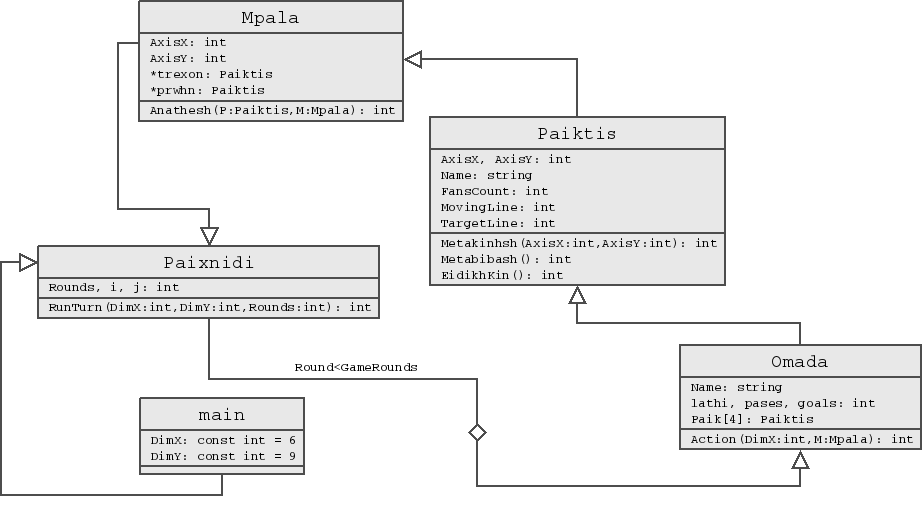
\includegraphics[width=16cm,keepaspectratio]{uml-c++2}
%----------------------------------------------------------------------------------------
\end{document}